\documentclass[tikz,border=12pt]{standalone}
\usepackage[no-math]{fontspec}
\usepackage{xeCJK}
\usepackage[UTF8,fontset=none]{ctex}
\usepackage{tikz}
\usetikzlibrary{arrows.meta,positioning,fit,calc,decorations.pathreplacing,backgrounds}

\IfFontExistsTF{Times New Roman}{\setmainfont{Times New Roman}}{\setmainfont{TeX Gyre Termes}}
\IfFontExistsTF{Kaiti TC}{\setCJKmainfont[AutoFakeBold=3]{Kaiti TC}}
  {\IfFontExistsTF{Songti TC}{\setCJKmainfont[AutoFakeBold=3]{Songti TC}}
    {\setCJKmainfont{PingFang TC}}}

% thesis_colors.tex ─ 論文統一 TikZ 色票定義
% 在每個 standalone 圖的 preamble 以 % thesis_colors.tex ─ 論文統一 TikZ 色票定義
% 在每個 standalone 圖的 preamble 以 % thesis_colors.tex ─ 論文統一 TikZ 色票定義
% 在每個 standalone 圖的 preamble 以 \input{thesis_colors.tex} 引入

\definecolor{thesisBlue}{RGB}{43,108,176}      % 訓練集、主箭頭、主色
\definecolor{thesisAmber}{RGB}{201,140,30}     % 驗證集、次要強調
\definecolor{thesisCrimson}{RGB}{155,35,53}    % 測試集、警示
\definecolor{thesisTeal}{RGB}{74,157,143}      % 節點類型 1（電子零組件）
\definecolor{thesisForest}{RGB}{45,122,79}     % 節點類型 2（光電及I/O）、LSTM Update
\definecolor{thesisSand}{RGB}{194,168,120}     % 節點類型 3（半導體）
\definecolor{thesisDark}{RGB}{45,55,72}        % 框線、文字、主箭頭
\definecolor{thesisLight}{RGB}{237,242,247}    % 淡背景、節點填色
\definecolor{thesisPurple}{RGB}{107,70,193}    % GAT 第二注意力頭
\definecolor{thesisMidGray}{RGB}{130,145,160}  % 次要線段、虛線
 引入

\definecolor{thesisBlue}{RGB}{43,108,176}      % 訓練集、主箭頭、主色
\definecolor{thesisAmber}{RGB}{201,140,30}     % 驗證集、次要強調
\definecolor{thesisCrimson}{RGB}{155,35,53}    % 測試集、警示
\definecolor{thesisTeal}{RGB}{74,157,143}      % 節點類型 1（電子零組件）
\definecolor{thesisForest}{RGB}{45,122,79}     % 節點類型 2（光電及I/O）、LSTM Update
\definecolor{thesisSand}{RGB}{194,168,120}     % 節點類型 3（半導體）
\definecolor{thesisDark}{RGB}{45,55,72}        % 框線、文字、主箭頭
\definecolor{thesisLight}{RGB}{237,242,247}    % 淡背景、節點填色
\definecolor{thesisPurple}{RGB}{107,70,193}    % GAT 第二注意力頭
\definecolor{thesisMidGray}{RGB}{130,145,160}  % 次要線段、虛線
 引入

\definecolor{thesisBlue}{RGB}{43,108,176}      % 訓練集、主箭頭、主色
\definecolor{thesisAmber}{RGB}{201,140,30}     % 驗證集、次要強調
\definecolor{thesisCrimson}{RGB}{155,35,53}    % 測試集、警示
\definecolor{thesisTeal}{RGB}{74,157,143}      % 節點類型 1（電子零組件）
\definecolor{thesisForest}{RGB}{45,122,79}     % 節點類型 2（光電及I/O）、LSTM Update
\definecolor{thesisSand}{RGB}{194,168,120}     % 節點類型 3（半導體）
\definecolor{thesisDark}{RGB}{45,55,72}        % 框線、文字、主箭頭
\definecolor{thesisLight}{RGB}{237,242,247}    % 淡背景、節點填色
\definecolor{thesisPurple}{RGB}{107,70,193}    % GAT 第二注意力頭
\definecolor{thesisMidGray}{RGB}{130,145,160}  % 次要線段、虛線


\begin{document}
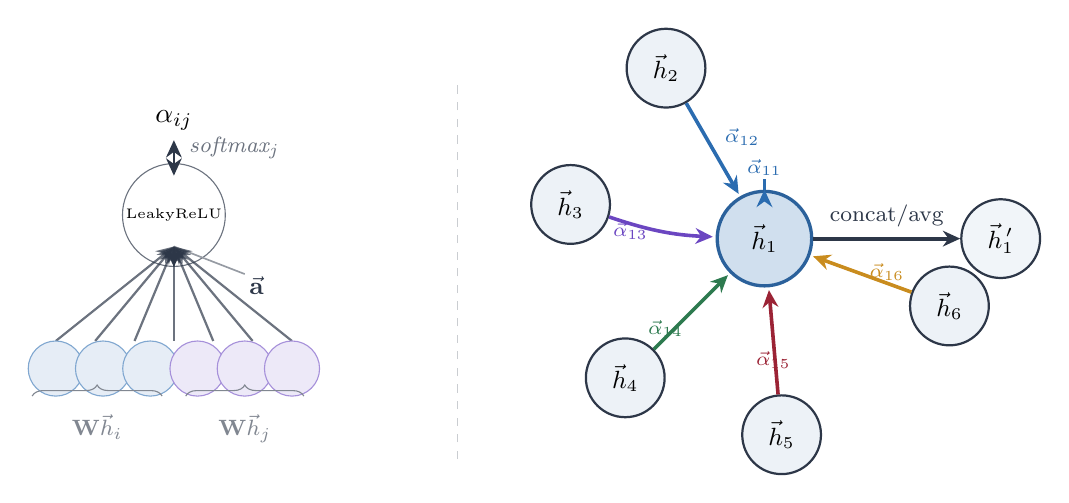
\begin{tikzpicture}[
  gnode/.style={circle, draw=thesisDark, fill=thesisLight, thick, minimum size=10mm,
                font=\small},
  centernode/.style={circle, draw=thesisBlue!80!thesisDark, fill=thesisBlue!22,
                     very thick, minimum size=12mm, font=\small\bfseries},
  outputnode/.style={circle, draw=thesisDark, fill=thesisLight!80, thick,
                     minimum size=10mm, font=\small},
  actnode/.style={circle, draw=thesisDark!70, fill=white, thin, minimum size=9mm,
                  font=\small, inner sep=1pt},
  arr/.style={-{Stealth[length=2.2mm,width=2mm]}, thick},
  darkarr/.style={arr, thesisDark},
  thinwire/.style={thesisDark!50, line width=0.6pt},
]

%%──────────────────────────────────────────────────────────────────
%% LEFT PANEL: Attention coefficient calculation
%%──────────────────────────────────────────────────────────────────
\def\lx{0}

% Result at top: α_ij
\node[font=\normalsize] (aij) at (\lx, 5.8) {$\alpha_{ij}$};

% softmax arrow
\draw[darkarr] (\lx, 5.1) -- (aij.south);
\node[font=\footnotesize\itshape, thesisDark!70, right=2pt] at (\lx, 5.45)
      {softmax${}_j$};

% LeakyReLU / activation circle
\node[actnode] (act) at (\lx, 4.6) {\tiny LeakyReLU};
\draw[darkarr] (\lx, 4.2) -- (act.south);
\draw[darkarr] (act.north) -- (\lx, 5.1);

% shared attention vector a label
\node[font=\small, thesisDark] (alabel) at (\lx+1.05, 3.7) {$\vec{\mathbf{a}}$};
\draw[thinwire] (\lx, 4.2) -- (\lx+0.9, 3.85);

% Fan-in arrows from feature nodes below
\foreach \dx in {-1.5,-1.0,-0.5,0,0.5,1.0,1.5}{
  \draw[darkarr, opacity=0.7] (\lx+\dx, 3.0) -- (\lx, 4.2);
}

% Bottom feature nodes: W*h_i (left group) and W*h_j (right group)
\foreach \k in {1,2,3}{
  \node[circle, draw=thesisBlue!60, fill=thesisBlue!12, minimum size=7mm,
        font=\footnotesize] at ({\lx-1.5+(\k-1)*0.6}, 2.65) {};
}
\foreach \k in {1,2,3}{
  \node[circle, draw=thesisPurple!60, fill=thesisPurple!12, minimum size=7mm,
        font=\footnotesize] at ({\lx+0.3+(\k-1)*0.6}, 2.65) {};
}

% Braces and labels
\draw[decorate, decoration={brace,amplitude=4pt}, thesisDark!60]
     ({\lx-1.8}, 2.3) -- ({\lx-0.15}, 2.3)
     node[midway, below=3pt, font=\footnotesize]{$\mathbf{W}\vec{h}_i$};
\draw[decorate, decoration={brace,amplitude=4pt}, thesisDark!60]
     ({\lx+0.15}, 2.3) -- ({\lx+1.65}, 2.3)
     node[midway, below=3pt, font=\footnotesize]{$\mathbf{W}\vec{h}_j$};

% Separator line
\draw[thesisDark!25, dashed, thin] (3.6, 1.5) -- (3.6, 6.3);

%%──────────────────────────────────────────────────────────────────
%% RIGHT PANEL: Radial neighbor aggregation
%%──────────────────────────────────────────────────────────────────
\def\rx{7.5}   % x center
\def\ry{4.3}   % y center
\def\R{2.5}    % radius

% Central node h_1 (bold blue)
\node[centernode] (h1) at (\rx, \ry) {$\vec{h}_1$};

% Six surrounding neighbor nodes at angles (starting top, going CW)
% h2: 125° h3: 160° h4: 225° h5: 270° h6: 315° (and h1 self at ~70°)
\node[gnode] (h2) at ({(\rx)+\R*cos(120)}, {(\ry)+\R*sin(120)}) {$\vec{h}_2$};
\node[gnode] (h3) at ({(\rx)+\R*cos(170)}, {(\ry)+\R*sin(170)}) {$\vec{h}_3$};
\node[gnode] (h4) at ({(\rx)+\R*cos(225)}, {(\ry)+\R*sin(225)}) {$\vec{h}_4$};
\node[gnode] (h5) at ({(\rx)+\R*cos(275)}, {(\ry)+\R*sin(275)}) {$\vec{h}_5$};
\node[gnode] (h6) at ({(\rx)+\R*cos(340)}, {(\ry)+\R*sin(340)}) {$\vec{h}_6$};

% Attention edges: colored arrows + α labels
% α_11 (self-loop): top of center node
\draw[arr, thesisBlue, line width=1.4pt, looseness=6, in=50, out=130]
      (h1.north) to
      node[pos=0.5, font=\scriptsize, thesisBlue, above=1pt] {$\vec{\alpha}_{11}$}
      (h1.north);

\draw[arr, thesisBlue, line width=1.3pt, shorten >=1pt] (h2) to
      node[pos=0.55, font=\scriptsize, thesisBlue, above right=-1pt] {$\vec{\alpha}_{12}$}
      (h1);
\draw[arr, thesisPurple, line width=1.3pt, shorten >=1pt, bend right=8] (h3) to
      node[pos=0.5, font=\scriptsize, thesisPurple, left=1pt] {$\vec{\alpha}_{13}$}
      (h1);
\draw[arr, thesisForest, line width=1.3pt, shorten >=1pt] (h4) to
      node[pos=0.5, font=\scriptsize, thesisForest, below left=-1pt] {$\vec{\alpha}_{14}$}
      (h1);
\draw[arr, thesisCrimson, line width=1.3pt, shorten >=1pt] (h5) to
      node[pos=0.5, font=\scriptsize, thesisCrimson, below] {$\vec{\alpha}_{15}$}
      (h1);
\draw[arr, thesisAmber, line width=1.3pt, shorten >=1pt] (h6) to
      node[pos=0.55, font=\scriptsize, thesisAmber, right=1pt] {$\vec{\alpha}_{16}$}
      (h1);

% Output arrow: concat/avg → h'_1
\node[outputnode] (h1p) at ({\rx+3.0}, \ry) {$\vec{h}^{\,\prime}_1$};
\draw[darkarr, line width=1.5pt] (h1.east) -- (h1p.west)
      node[midway, above, font=\footnotesize] {concat/avg};

\end{tikzpicture}
\end{document}
